\chapter{Topology}\label{chapter:topology.2}
\chapterSummary{%%
We define topological spaces and their essential properties.}%%

\section{Motivation}
When we study polynomial functions on the plane, there is a natural notion of ``open set'' different from the usual one: a \emph{Zariski open set}\define{open!set!Zariski}\define{Zariski!topology}\define{topology!Zariski}\define{Zariski!open set} is the set of points on which some polynomial function \(p\) is not zero.
For example, 
\[
U=\set{(x,y)\in \R{2}|x^2+y \ne 0}
\]
is a Zariski open set.
Of course, \(U\) is also an open set in the usual sense, but
\[
W=\set{(x,y)\in\R{2}|x>0}
\]
is an open set in the usual sense, but not a Zariski open set.
\begin{problem}{topology:Z.inequality}
Prove that \(W\) is not Zariski open.
\end{problem}
So we can have different concepts of open set playing different but no less useful roles in the same space \(\R{2}\).
Intuitively, an open set is like a little ``fat blob''.
If you want to study polynomial functions, then sets like \(W\) above are not as fat as they ``should'' be, because any polynomial which doesn't vanish on \(W\) \emph{also} doesn't vanish on some much larger set.

\section{Definition}
A \emph{topology}\define{topology} on a set \(X\) is a collection of subsets of \(X\), called the \emph{open sets}\define{open!set}\define{set!open} of the topology, so that
\begin{enumerate}
\item the union of any collection of open sets is an open set,
\item the intersection of any finite collection of open sets is an open set,
\item the empty set and the whole of \(X\) are open sets.
\end{enumerate}
A \emph{topological space}\define{space!topological}\define{topological space} is a set \(X\) equipped with a topology; we usually leave the topology as implicitly understood somehow.
The elements of the set \(X\) are called \emph{points}.\define{point}
\begin{example}
As in our previous experience, every subset \(X \subseteq \R{n}\) is a topological space, with open sets being the intersections \(X\cap U\) where \(U \subseteq \R{n}\) is the union of a collection of open balls, the \emph{Euclidean topology}.
If no topology is otherwise specified, we always mean the Euclidean topology.
\end{example}
\begin{example}
If \(X\) is a metric space, then the usual open sets (unions of open balls) form a topology, making every metric space into a topological space, its \emph{metric topology}.
If no topology is otherwise specified, we always mean the metric topology.
\end{example}
\begin{example}
Take any set \(X\) and let the open sets be all of the subsets of \(X\), the \emph{discrete topology}.\define{topology!discrete}\define{discrete!topology}
\end{example}
\begin{example}
Take any set \(X\) and let the only open sets be the empty set and \(X\), the \emph{indiscrete topology}.\define{topology!indiscrete}\define{indiscrete!topology}
\end{example}
\begin{example}
Take \(X=\R{n}\) and take as open sets the sets
\[
\set{x \in \R{n}|p(x) \ne 0}
\]
for some polynomial function \(p\) on \(\R{n}\): the \emph{Zariski topology}.
\end{example}
\begin{example}
The \emph{periodic topology} on \(X=\R{}\) is the topology whose open sets are just those from among the usual (Euclidean) topology which happen to be \(2\pi\) periodic.
\begin{center}
\documentclass[tikz]{standalone}
\begin{document}

\begin{tikzpicture}
\draw[gray!50, thick] (0,0) -- (8.5,0);
\newcount\j
\foreach \i in {-1,...,7}{ 
\j=\i
\draw[gray, very thick] ({1+\j},0) -- ({1.5+\j},0);
\draw[gray,thick,fill=white] ({1+\j},0) circle (1.8pt);
\draw[gray,thick,fill=white] ({1.5+\j},0) circle (1.8pt);
}
\end{tikzpicture}
\end{document}
\end{center}
\end{example}
\begin{example}
Let \(X\) be the set of nonnegative real numbers, and take as open sets all sets of the form 
\[
\set{x|x_0 < x},
\]
for any real number \(x_0 \ge 0\).
This is yet another topology.
\end{example}
\begin{example}
If \(S \subseteq X\) is any subset of a topological space, the \emph{subspace topology}%
\define{subspace!topology}\define{topology!subspace} on \(S\) has open sets \(S \cap U \subseteq S\) for \(U \subseteq X\) any open set.
\end{example}
\begin{example}
If \(X\) is any set, the \emph{cofinite topology}\define{cofinite topology}\define{topology!cofinite} has open sets just precisely (i) the empty set and (ii) the sets \(X-F\) where \(F\) is any finite set.
\end{example}
\begin{problem}{topology:check}
Check that each of these examples correctly defines a topology.
\end{problem}
\begin{problem}{topology:small.sets}
What are all topologies on the empty set? On a set with one element \(X=\set{0}\)? On a set with two elements \(X=\set{0,1}\)? On a set with three elements \(X=\set{0,1,2}\)? 
On a set with 4 elements \(X=\set{0,1,2,3}\)? 
\end{problem}
\begin{answer}{topology:small.sets}
On the empty set, the only topology is the one whose only open set is the empty set.
On the set \(X=\set{0}\), the only topology is the discrete topology, which is also the indiscrete topology.
On the set \(X=\set{0,1}\), the possible topologies are
\begin{enumerate}
\item discrete: open sets are: the empty set, \(\set{0},\set{1},\set{0,1}\);
\item indiscrete: open sets are: the empty set, \(\set{0,1}\);
\item the \emph{Sierpinski topology}: open sets are: the empty set, \(\set{0}, \set{0,1}\);
\item the \emph{other Sierpinski topology}: open sets are: the empty set, \(\set{1}, \set{0,1}\).
\end{enumerate}
\end{answer}
\begin{example}
Take distinct points \(p, q\), let \(r\) be the distance between them, and look at the balls of radius \(r/2\) around those points.
Those balls are not empty, but don't intersect.
Hence any metric space with two or more points contains nonintersecting nonempty open sets.
\end{example}
\begin{example}
If we take nonempty Zariski open sets \(U,W \subseteq \R{n}\), we claim they intersect.
Write
\[
U=\set{x \in \R{n}|p(x) \ne 0}
\]
and
\[
W=
\set{x \in \R{n}|q(x) \ne 0}.
\]
We need to find a point in \(U\cap W\), i.e. a point where neither of these polynomials vanish.
Since \(U\) and \(W\) are not empty, we can take points \(x\) in \(U\) and \(y\) in \(W\).
Take the line between them.
It is enough to find a point of that line on which neither of those polynomials vanish.
We can rotate and translate to get that line to the \(x_1\)-axis.
Set all of the other variables except \(x_1\) to zero.
So it is enough to assume that both of our polynomials depend on only one variable.
Each polynomial, being not everywhere zero, vanishes on a finite set of points.
Remove those points, and neither of the polynomials vanish on any of the remaining points: \(U\) and \(W\) contain a point in common.
Therefore the Zariski topology is \emph{not} a metric topology of \emph{any} metric (including, in particular, the usual metric).
\end{example}

\section{Closed sets}
If \(A\) is a subset of a set \(B\), we write \(B-A\) to mean the set of points of \(B\) not lying in \(A\), the \emph{complement}\define{complement} of \(A\) in \(B\).
A subset \(C \subseteq X\) of a topological space \(X\) is \emph{closed}\define{closed!set}\define{set!closed} if its complement \(X - C \subseteq X\) is open.
\begin{problem}{topology:closed.properties}
Prove that the intersection of any closed sets is closed.
\end{problem}
\begin{answer}{topology:closed.properties}
Take some sets \(\set{C_a}_{a \in \mathcal{A}}\), so that each \(C_a \subseteq X\) is closed.
The complement \(U_a\defeq X-C_a\) is open.
So the union \(U \defeq \bigcup_a U_a\) is open.
So its complement \(C=X-U\) is closed.
But \(C\) is the set of points of \(X\) not belonging to \(U\), i.e. not belonging to any \(U_a\), i.e. belonging to \(C_a\) instead of \(U_a\) for every \(a\), i.e. \(C=\bigcap_a C_a\).
\end{answer}
\begin{problem}{topology:closed.properties.2}
Prove that union of finitely many closed sets is closed.
\end{problem}
\begin{problem}{topology:closed.properties.3}
Prove that the empty set and \(X\) are closed subsets of any topological space \(X\).
In particular, sets can be \emph{both} open and closed (sets are \emph{not} doors).
\end{problem}
The \emph{closure}\define{closure} \(\bar{A}\) of a set \(A \subseteq X\) in a topological space \(X\) is the intersection of all closed sets containing \(A\).
\begin{problem}{topology:closure.1}
Find the closure of the rational numbers in the real numbers.
\end{problem}
\begin{problem}{topology:closure.2}
Find the closure of the open unit ball in \(\R{n}\).
\end{problem}
\begin{problem}{topology:closure.4}
Find the closure of the open unit ball in \(\R{n}\) with the Zariski topology.
\end{problem}
\begin{problem}{topology:closure.5}
Prove that 
\begin{enumerate}
\item
the closure \(\bar{A}\) of any subset \(A \subseteq X\) of any topological space \(X\) is closed
\item
\(A\) is closed just when \(A=\bar{A}\)
\item
\(A \subseteq \bar{A}\)
\item
\(\bar{A}\) lies inside any closed set containing \(A\).
\end{enumerate}
\end{problem}

\section{Bases}
A \emph{neighborhood}\define{neighborhood} of a point \(x \in X\) in a topological space is a subset \(S \subseteq X\) containing \(x\) so that there is an open subset \(U \subseteq X\) lying inside \(S\) and containing \(x\).
A \emph{basis}\define{basis!topology}\define{topology!basis} is a collection of open sets so that every open set is a union of open sets from the basis.
\begin{example}
The open balls of a metric space form a basis for the metric topology.
\end{example}
\begin{example}
The only basis of the cofinite topology on any infinite set is the entire cofinite topology.
\end{example}
\begin{example}
All open sets taken together form a basis (there is no reasonable notion here of ``independence'' like in linear 
algebra).
\end{example}
\begin{problem}{topology:basis.shrink}
Prove that every basis \(S\) of \(\R{n}\) contains an infinite set \(T \subset S\) so that \(S - T\) is also a basis.
\end{problem}
\begin{problem}{topology:basis.characterize}
A collection of open sets of a topological space \(X\) forms a basis just when, for any point \(x \in X\) and neighborhood \(N \subseteq X\) of \(x\), there is an element \(U\) in that collection so that \(x \in U \subseteq N\).
\end{problem}
\begin{problem}{topology:basis.rn}
Prove that the topology of \(\R{n}\) has a countable basis.
\end{problem}
\begin{problem}{topology:basis.rn.zariski}
Prove that the Zariski topology on \(\R{n}\) does not have a countable basis.
Hint: first try \(n=1\).
\end{problem}
\begin{problem*}{topology:basis.weird}
Give an example of an open set \(U \subseteq \R{}\) containing the rational numbers so that \(\R{}- U\) is uncountable.
\end{problem*}
A \emph{basis} \(S\) on a set \(X\) is a collection of subsets of \(X\) so that any finite intersection of those subsets is also expressible as a union of some of those subsets.
Clearly \(S\) is a then a basis for a unique topology: the one whose open sets are unions of any collections of those subsets, called the topology \define{generated} by or \define{spanned} by \(S\).

\section{Boundaries}
Given a subset \(A \subseteq X\) of a topological space, a point \(x \in X\) is an \emph{interior point}\define{interior} of \(A\) if \(A\) is a neighborhood of \(x\), an \emph{exterior point}\define{exterior} of \(A\) if \(X-A\) is a neighborhood of \(x\), and a \emph{boundary point}\define{boundary} otherwise, i.e. if every neighborhood of \(x\) contains points both inside \(A\) and outside \(A\).
The \emph{exterior} is the set of exterior points, and so on.
\begin{problem}{topology:interior}
Find the interior, exterior and boundary of
\begin{enumerate}
\item the set \(A \subset X\) of rational numbers inside the set \(X\) of real numbers.
\item the set \(A \subset X\) of irrational numbers inside the set \(X\) of real numbers.
\item the set \(A \subset X\) of positive numbers inside the set \(X\) of real numbers.
\item the set \(A \subset X\) of positive numbers inside the set \(X\) of rational numbers.
\item the unit interval \(A \subset X\) inside the set of \(X=\R{}\) in the Zariski topology.
\item the rational numbers \(A \subset X\) inside the set of \(X=\R{}\) in the Zariski topology.
\end{enumerate}
\end{problem}
\begin{problem}{topology:interior.1}
Find a subset \(A \subset \R{}\) whose boundary has nonempty interior.
\end{problem}
\begin{problem}{topology:interior.2}
Take any set \(X\) with the discrete topology and any subset \(A \subseteq X\).
Find the interior, exterior and boundary of \(A\).
\end{problem}
\begin{problem}{topology:interior.3}
Take any set \(X\) with the indiscrete topology and any subset \(A \subseteq X\).
Find the interior, exterior and boundary of \(A\).
\end{problem}
\begin{problem}{topology:3.sets.same.boundary}
Find 3 different open subsets of the real number line that have the same boundary.
\end{problem}
\begin{problem}{topology:boundary.points}
Suppose that \(U\) is an open subset of the plane and that the boundary of \(U\) is a finite set of points, say \(\set{p_1,p_2,\dots,p_k}\).
Prove that \(U=\R{2}-\set{p_1,p_2,\dots,p_k}\).
\end{problem}

\section{Density}
A subset \(A \subseteq X\) of a topological space is \emph{dense}\define{dense} in a subset \(B \subset X\) if \(B \subset \bar{A}\), and \emph{everywhere dense} if \(\bar{A}=X\).
\begin{problem}{topology:dense}
Prove that every nonempty open set in \(\R{n}\) in the Zariski topology is everywhere dense.
\end{problem}
\begin{problem}{topology:dense.q}
Prove that the rational numbers are dense in the real numbers.
\end{problem}
\begin{example}
In the indiscrete topology, every nonempty subset is everywhere dense.
\end{example}
\begin{example}
In the discrete topology on a set \(X\), only \(X\) is everywhere dense.
\end{example}
\begin{example}
In \(\R{n}\), the points with rational coordinates are everywhere dense, as are the points with irrational coordinates.
\end{example}
\begin{problem}{topology:dense.closure}
If \(A \subset X\) is dense and \(U \subset X\) is open, prove that \(A \cap U\) is dense in \(U\).
\end{problem}

\section{Separability}
A topological space \(X\) is \emph{separable} if it contains a dense sequence of points, i.e. a sequence which enters every open set.
\begin{example}
In the indiscrete topology, every sequence is dense, so the space is separable.
\end{example}
\begin{example}
In the discrete topology on a set \(X\), only \(X\) is everywhere dense, so if the points of \(X\) do not all lie on a single sequence, then \(X\) is not separable.
\end{example}
\begin{example}
The real numbers are separable: put the rational numbers into a sequence.
\end{example}
\begin{example}
Euclidean space is separable: put the points with rational coordinates into a sequence.
\end{example}
\begin{problem}{topology:separ}
Which of the following topologies on \(\R{n}\) make \(\R{n}\) separable?
\begin{enumerate}
\item
The Euclidean topology.
\item
The discrete topology.
\item
The cofinite topology.
\item
The Zariski topology.
\end{enumerate}
\end{problem}
\begin{problem*}{topology:half.open}
The \emph{half-open topology}\define{half-open topology}\define{topology!half-open} on \(\R{}\) is the topology generated by the half intervals \(a \le x < b\) for numbers \(a < b \in \R{}\).
Prove that this topology has a countable basis, is separable, and is \emph{not} the Euclidean topology.
\end{problem*}

\section{Products}
Recall that the plane \(\R{2}\) is the product \(\R{2} = \R{} \times \R{}\).
But the open sets of the plane are not all products; there are disks, interiors of triangles, and so on, as well.
\begin{center}
\documentclass[tikz]{standalone}
\usepackage{calc}
\begin{document}
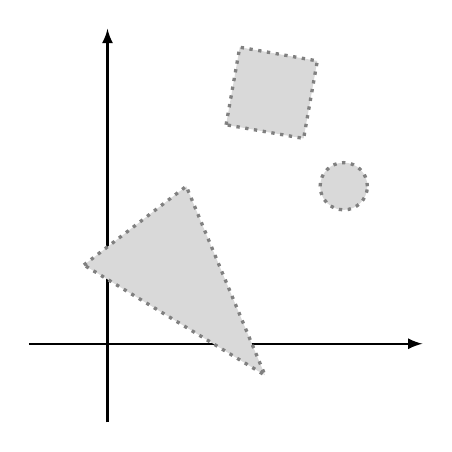
\begin{tikzpicture}
\draw[thick, black, -latex] (-1,0) -- (4,0);
\draw[thick, black, -latex] (0,-1) -- (0,4);
\fill[gray!30,very thick, draw=gray, dotted] (-.3,1) -- (1,2) -- (2,-.4) -- cycle;
\fill[gray!30,very thick, draw=gray, dotted] (3,2) circle (.3);
\fill[gray!30,very thick, draw=gray, dotted, cm={cos(10) ,-sin(10) ,sin(10) ,cos(10) ,(0 cm,0 cm)}] (1,3) -- (1,4) -- (2,4) -- (2,3) -- cycle;
\end{tikzpicture}
\end{document}

\end{center}
The product open sets in the plane are only the products of intervals, i.e. the open boxes:
\begin{center}
\documentclass[tikz]{standalone}
\usepackage{calc}
\begin{document}
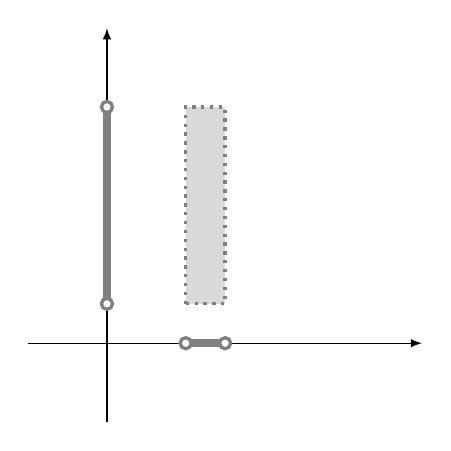
\begin{tikzpicture}
\draw[black, -latex] (-1,0) -- (4,0);
\draw[black, -latex] (0,-1) -- (0,4);
\draw[line width=3pt, gray] (0,.5) -- (0,3);
\draw[line width=3pt, gray] (1,0) -- (1.5,0);
\fill[white,draw=gray,very thick] (0,.5) circle (2pt);
\fill[white,draw=gray,very thick] (0,3) circle (2pt);
\fill[white,draw=gray,very thick] (1,0) circle (2pt);
\fill[white,draw=gray,very thick] (1.5,0) circle (2pt);
\fill[gray!30,very thick, draw=gray, dotted] (1,.5) -- (1.5,.5) -- (1.5,3) -- (1,3) -- cycle;
\end{tikzpicture}
\end{document}

\end{center}
If \(X\) and \(Y\) are topological spaces, the \emph{product topology}\define{topology!product}\define{product!toplogy} on \(X \times Y\) has as open sets precisely those sets whose every point lies in a product \(U_X \times U_Y\) of an open set \(U_X \subset X\) and an open set \(U_Y \subset Y\).
\begin{problem}{topology:products.1}
Take any basis for the topology of \(X\), and any basis for the topology of \(Y\).
Take the open sets of the form of a product \(U_X \times U_Y\) of a basis element \(U_X \subset X\) and a basis element \(U_Y \subset Y\).
Prove that these form a basis for the product topology.
\end{problem}
\begin{problem}{topology:products.closed}
Suppose that \(A \subset X\) and \(B \subset Y\) are closed sets in topological spaces.
Prove that \(A \times B\) is a closed set in \(X \times Y\) in the product topology.
\end{problem}
\begin{problem}{topology:products.open}
Suppose that \(A \subset X\) and \(B \subset Y\) are sets in topological spaces and write \(A^{\circ}\) for the interior of a set and \(\bar{A}\) for its closure.
Prove that \(\pr{A \times B}^{\circ}=A^{\circ} \times B^{\circ}\) and that \(\bar{A} \times \bar{B}=\overline{A \times B}\) in the product topology.
\end{problem}
\begin{problem}{topology:products.Zariski}
If \(X=\R{p}\) and \(Y=\R{q}\) with the Zariski topology, is the product topology on \(X \times Y=\R{p+q}\) equal to the Zariski topology on \(\R{p+q}\)?
\end{problem}


\section{Subspaces}
If \(A \subset X\) is a subset of a topological space \(X\), the \emph{subspace topology}\define{topology!subspace}\define{subspace!topology} has as open sets the sets \(A \cap U\) for any open set \(U \subset X\).
\begin{problem}{topology:subspaces}
Prove that the subspace topology is a topology.
\end{problem}
\begin{problem*}{topology:sep.sub}
If a topological space is separable, is every subset separable in its subspace topology?
\end{problem*}
\begin{problem}{topology:a.b.c}
Suppose that \(A \subset B \subset X\) are subsets of a topological space.
Then \(A\) has a subspace topology as a subset of \(X\), as does \(B\).
But then \(A\) has another subspace topology, as a subspace of \(B\) where \(B\) has its subspace topology as a subspace of \(X\).
Prove that these two topologies on \(A\) are the same topology.
\end{problem}
\begin{example}
If \(X=\R{}\) and \(A=\R{> 0}\), then the closure of \(A\) as a subset of \(A\) is \(A\), but as a subset of \(X\) the closure of \(A\) inside \(X\) is \(\R{\ge 0}\).
\end{example}
\begin{lemma}
If \(A \subset X\) is a subset of a topological space \(X\), then \(A\) has as closed sets just exactly the sets \(A \cap C\) for any closed set \(C \subset X\).
Moreover, the closure of a subset \(S \subset A\) inside \(A\) is the intersection of \(A\) with the closure of \(S\) in \(X\).
\end{lemma}
\begin{proof}
Take a subset \(S \subset A\) and let \(C_X \subset X\) be its closure in \(X\) and \(C_A \subset A\) be its closure in \(A\).
Let \(U_A = A - C_A\) and \(U_X = X - C_X\).
Then 
\[
C_A = \bigcap_{S \subset C} C
\]
where the intersection is over the \(A\)-closed subsets of \(A\) containing \(S\).
So
\begin{align*}
U_A 
&= 
A - C_A,
\\
&=
\bigcap_{S \cap U\text{ empty}} U,
\\
\intertext{where the intersection is over the \(A\)-open sets \(U \subset A\) not intersecting \(S\); write those open sets  as \(U \cap A\), for \(X\)-open sets \(U \subset X\):}
&=
\bigcap_{S \cap U \cap A\text{ empty}} U \cap A,
\\
\intertext{but then \(S \cap U \cap A=S \cap U\) since \(S \subset A\), so}
&=
\bigcap_{S \cap U\text{ empty}} U \cap A,
\\
\intertext{where the intersection is over the \(X\)-open sets \(U \subset X\) not intersecting \(S\),}
&=
A \cap \bigcap_{S \cap U\text{ empty}} U,
\\
\intertext{where the intersection is over the \(X\)-open sets \(U \subset X\) not intersecting \(S\),}
&=
A \cap U_X.
\end{align*}
Therefore \(C_A = A \cap C_X\).
\end{proof}
\begin{problem}{topology:locally.closed}
A subset \(A \subset X\) of a topological space is \emph{locally closed}\define{locally!closed}\define{closed!locally} if each point \(a\) of \(A\) lies in an open subset \(U \subset X\) of \(X\) so that \(A \cap U \subset U\) is a closed subset of \(U\).
Given an example of a locally closed subset of \(X=\R{}\) which is not closed.
Given an example of a locally closed subset of \(X=\R{3}\) which is not closed.
\end{problem}
The \emph{disjoint union}\define{disjoint union} of two topological spaces \(X, Y\) is the set \(X \sqcup Y\) of all points of the form \((x,1)\) for \(x \in X\) or \((y,2)\) for \(y \in Y\).
We give it the topology for which a basis of open sets consists of sets of the form \(U \sqcup W\) for \(U \subset X\) open and \(W \subset Y\) open.
Intuitively, \(X \sqcup Y\) means \(X\) and \(Y\) ``drawn separated from one another''.
Typically, we will denote points of \(X\sqcup Y\) as \(x \in X\) or \(y \in Y\) rather than as pairs \((x,1)\) or \((y,2)\), as long as this doesn't confuse matters.

\section{Hausdorff}
Two point \(x,y \in X\) of a topological space \(X\) are \emph{housed off}\define{housed off} from one another if there are open sets \(U,V \subset X\) with \(x \in U\), \(y \in V\) and \(U\cap V\) is empty.
\begin{center}
\documentclass[tikz]{standalone}
\begin{document}
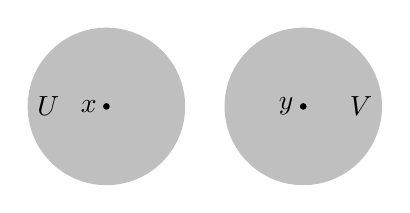
\begin{tikzpicture}
\fill[gray!50] (0,0) circle (1cm);
\node[right] at (-1,0) {\(U\)};
\fill (0,0) circle(1.2pt) node[left] {\(x\)};
\fill[gray!50] (2.5,0) circle (1cm);
\node[left] at (3.5,0) {\(V\)};
\fill (2.5,0) circle(1.2pt) node[left] {\(y\)};
\end{tikzpicture}
\end{document}

\end{center}
If any two distinct points of \(X\) are housed off, then \(X\) is \emph{Hausdorff}.\define{Hausdorff}
\begin{problem}{topology:cofinite.haus}
If \(X\) is any set with the cofinite topology, prove that \(X\) is Hausdorff just when \(X\) is finite.
\end{problem}
\begin{problem}{topology:metric.space.haus}
Prove that every metric space is Hausdorff.
\end{problem}
\begin{lemma}
The Zariski topology is not Hausdorff.
\end{lemma}
\begin{proof}
Take two points \(x, y \in \R{n}\) and two Zariski open sets \(U, V\) with \(x \in U\) and \(y \in V\).
We write \(U\) as the set of points at which some polynomial \(p\) doesn't vanish, and \(V\) as the set of points at which some polynomial \(q\) doesn't vanish.
Draw the line from \(x\) to \(y\).
Restrict the polynomials to that line.
None of our polynomials vanishes everywhere on that line, since each is nonzero at \(x\) or at \(y\).
So each vanishes at only a finite number of points.
Remove those points to see that \(U\) and \(V\) intersection.
\end{proof}
\begin{problem}{topology:closed.house}
Prove that in any Hausdorff space \(X\), for any point \(x\) of \(X\), the set \(\set{x}\) is closed: ``points are closed''.
\end{problem}
\begin{problem}{topology:closed.house.2}
Prove that, in the Zariski topology, ``points are closed'', even though the Zariski topology is not Hausdorff.
\end{problem}
\begin{problem}{topology:closed.house.3}
Prove that in any topological space, ``points are closed'' if and only if finite sets are closed.
\end{problem}
If \(X\) is a topological space, the \emph{diagonal}\define{diagonal}\Notation{DX}{\Delta_X}{diagonal} \(\Delta_X \subset X \times X\) be , i.e. the set of points \((x,x)\) for \(x\) in \(X\).
\begin{problem*}{topology:diagonal}
A topological space is Hausdorff just when its diagonal is closed.
\end{problem*}
\begin{answer}{topology:diagonal}
The diagonal is closed just when its complement is open.
Its complement is the set \(U \subset X \times X\) of pairs of distinct points.
This \(U\) is open just when every point of \(U\) lies inside a basis element which lies in \(U\), for any basis, and in particular for the basis consisting of products \(U_1 \times U_2\) of open sets \(U_1, U_2 \subset X\).
So the diagonal is closed just when, for any pair of distinct points \(x_1 \ne x_2\) in \(X\), the point \((x_1,x_2)\) lies inside a subset \(U_1 \times U_2 \subset X \times X\) which does not intersect the diagonal.
In other words, just when \(x_1 \in U_1\) and \(x_2 \in U_2\) but \(U_1 \cap U_2\) is empty.
In other words, just when \(X\) is Hausdorff.
\end{answer}
\begin{problem}{topology:product.Zariski.closure}
If \(X=\R{n}\) with the Zariski topology, prove that the diagonal in \(X \times X\) is dense in the product topology, but not in the Zariski topology on \(\R{2n}\).
\end{problem}
\begin{problem}{topology:product.Hausdorff}
The product \(X \times Y\) of two Hausdorff spaces \(X, Y\) is also a Hausdorff space.
\end{problem}
\begin{answer}{topology:product.Hausdorff}
Take two points \((x_1,y_1), (x_2,y_2)\) in \(X \times Y\).
Take disjoint open sets \(X_1, X_2 \subset X\) and \(Y_1, Y_2 \subset Y\) so that \(x_1, x_2, y_1, y_2\) belong to \(X_1, X_2, Y_1, Y_2 \) respectively.
Then \((x_1,y_1)\) is in \(X_1 \times Y_1\) and so on.
\end{answer}
\begin{problem}{topology:subspace.Hausdorff}
Prove that, for any subset \(A \subset X\) of a Hausdorff space, \(A\) is Hausdorff in the subspace topology on \(A\).
\end{problem}

\section{Compactness}
Recall that a subset \(A \subset \R{n}\) is compact just when every infinite sequence of points has a convergent subsequence.
We will try (and fail) to imitate this in topological spaces.
A sequence \(x_1, x_2, \dots\) of points of a topological space \(X\) \emph{converges}\define{convergence} to a point \(x \in X\) if every open set containing \(x\) contains all but finitely many points of that sequence.
\begin{example}
Take the sequence of points \(x_j=(j,2^j) \in \R{2}\) and let \(X=\R{2}\) with the Zariski topology.
Take any open set \(U\), not empty.
Then \(U\) has the form \(U=\R{2} - C\) where \(C \subset \R{2}\) is an algebraic curve in the plane (or \(C\) is the empty set).
Only finitely many points of our sequence can lie inside \(C\), because the points lie on the graph of \(y=2^x\), which is not an algebraic function.
(The reader should explain why that is the case.)
So, for any nonempty open set, all but finitely many points of our sequence lie in that open set.
In particular, this sequence converges to every point in the plane, in the Zariski topology.
\end{example}
Sequences turn out to be the wrong objects to work with in topology.
We work with open sets.

Recall another defining property of compact sets in \(\R{n}\): every open cover has a finite subcover.
An \emph{open cover}\define{open!cover}\define{cover!open} of a set \(A \subset X\) in a topological space \(X\) is a collection of open sets whose union contains \(A\).
A \emph{subcover} is a smaller collection of open sets, each one belonging the the original collection.
\begin{example}
The set of open balls of radius \(1/2\) is an open cover of the plane \(\R{2}\).
The subset of open balls of radius \(1/2\) with rational centre point is a subcover.
The set of open balls of radius \(1/3\) is \emph{not} a subcover: these balls are not drawn from our original set.
The set of open balls of radius \(1/2\) around integer points is not a subcover: the point \((1/2,1/2)\) is more than \(1/2\) unit from any integer point.
\end{example}
A topological space \(X\) is \emph{compact}\define{compact} if every open cover has a finite subcover.
\begin{problem}{topology:finite.compact}
Prove that every finite subset \(A \subset X\), of any topological space \(X\), is compact.
\end{problem}
\begin{lemma}
Every locally bounded function \(f \colon X \to \R{}\) on a compact topological space \(X\) is bounded.
\end{lemma}
\begin{proof}
Each point of \(X\) lies in an open set in which \(f\) is bounded.
These open sets cover \(X\).
Take a finite subcover.
So we have finitely many open sets, and a bound of \(f\) on each, from above and from below.
Take the maximum of the upper bounds, and minimum of the lower bounds.
\end{proof}
\begin{problem}{topological:compact.closed}
Suppose that \(A \subset X\) is a subset of a compact topological space.
Prove that if \(A\) is closed then \(A\) is compact.
If \(X\) is also Hausdorff, prove that \(A\) is closed just when \(A\) is compact.
\end{problem}
\begin{problem}{topological:compact.closed.2}
Give an example of a compact space \(X\) which is not Hausdorff and a compact set \(A \subset X\) which is not closed.
\end{problem}
\begin{answer}{topological:compact.closed.2}
Take \(X\) to be a set consisting of two points \(p,q\) with open sets: \(X\), the empty set, and the set \(\set{p}\).
Then \(\set{q}\) is the complement of \(\set{p}\), so closed.
But \(\set{p}\) is \emph{not} the complement of an open set, so is not closed.
There are only 4 open sets, so every open cover is finite.
\end{answer}
\begin{problem}{topological:compact.union}
Prove that, in any topological space, the union of finitely many compact sets is compact.
Give an example to prove that the union of infinitely many compact sets need not be compact.
\end{problem}
\begin{lemma}
Topological spaces \(X\) and \(Y\) are both compact just when their product is compact.
\end{lemma}
\begin{proof}
Suppose that \(X \times Y\) is compact.
Take an open cover \(X_a\) of \(X\).
Then \(X_a \times Y\) is an open cover of \(X \times Y\).
Take a finite subcover, say \(X_i \times Y\), \(i=1,2,\dots,n\).
Then \(X_1, X_2, \dots, X_n\) is a finite subcover of the collection of \(X_a\).
The same trick for \(Y\) in place of \(X\).

Suppose that \(X\) and \(Y\) are compact.
Take an open cover by open sets \(U_a \subset X \times Y\).
Each point \((x,y) \in X \times Y\) lies in one of these open sets, call it \(U_{x,y}\).
The product open sets \(X_b \times Y_c \subset X \times Y\) form a basis.
So there is such a product, call it \(X_{x,y} \times Y_{x,y}\), inside \(U_{x,y}\).

For each point \(x \in X\), the various \(Y_{x,y}\) cover \(Y\).
Take a finite subcover, say 
\[
Y_{x,y_1(x)}, \dots, Y_{x,y_{n_x}(x)}.
\]
Let
\[
X_x = X_{x,y_1(x)} \cap \dots \cap X_{x,y_{n_x}(x)}.
\]

Since \(x \in X_x\), these various open sets \(X_x \subset X\) form an open cover of \(X\).
Take a finite subcover \(X_1, X_2, \dots, X_n\), say containing points \(x_1 \in X_1, \dots, x_n \in X_n\).
Then \(X \times Y\) is covered by the finitely many sets
\(
U_{x_i,y_j(x_i)}
\)
for all possible values of \(i\) and \(j\) for which this is defined.
\end{proof}
\begin{lemma}\label{lemma:compact.closed}
In any Hausdorff space, every compact set is closed.
\end{lemma}
\begin{proof}
Suppose that \(X\) is Hausdorff.
Since \(X\) is Hausdorff, any two points \(x,y \in X\) have disjoint ``houses''.
Suppose that \(x\) is outside a compact set \(K \subseteq X\).
Fixing \(x\) and letting \(y\) vary over \(K\), finitely many of our ``houses'' cover those points of \(K\).
The finite intersection of the corresponding ``houses'' around \(x\) give an open set around \(x\) not intersecting \(K\).
So every point \(x\) outside \(K\) lies in an open set outside \(K\), i.e. the complement of \(K\) is open.
\end{proof}
\begin{problem}{topology:Hausdorff.locally}
Give an example of a compact but not closed subset of some non-Hausdorff space.
\end{problem}
\begin{problem}{topology:Hausdorff.compact.intersection}
Prove that, in any Hausdorff space, for any collection of compact sets, the intersection of all of those sets is compact.
If the intersection of any finite number of those compact sets is not empty, prove that the intersection of them all is not empty.
\end{problem}
\begin{answer}{topology:Hausdorff.compact.intersection}
Take compact sets \(K_a\) and let \(K\) be their intersection.
Take an open cover \(U_b\) of \(K\).
By lemma~\vref{lemma:compact.closed}, every \(K_a\) is closed.
Therefore the intersection \(K\) is closed, so \(X-K\) is open.
The open sets \(\set{X-K} \cup \set{U_b}\) cover \(X\).
So each set \(K_a\) is covered by these, and so covered by finitely many of these.
But then those finitely many cover \(K \subset K_a\).
So \(K\) is compact.
Suppose that \(K\) is empty.
The open sets \(W_b \defeq X-K_b\) cover \(X\).
Each set \(K_a\) is compact, so finitely many \(W_b\) cover \(K_a\), say \(W_{b_1}, \dots, W_{b_n}\).
So \(W_a, W_{b_1}, \dots, W_{b_n}\) covers \(X\).
So their complements \(K_a, K_{b_1},\dots,K_{b_n}\) intersect in an empty set.
\end{answer}
\begin{problem}{topology:not.Hausdorff.compact.intersection}
Give an example of a space, not Hausdorff, and two compact subsets of that space, whose intersection is not compact.
\end{problem}
\begin{answer}{topology:not.Hausdorff.compact.intersection}
Let \(X=\set{0,1,2,\dots}\cup\{\infty,\infty'\}\), where a subset \(U\subseteq X\) is open just when either \(U\subseteq\set{0,1,2,\dots}\) or \(X\setminus U\) is finite.  Then \(A=\set{0,1,2,\dots}\cup\{\infty\}\) and \(B=\set{0,1,2,\dots}\cup\{\infty'\}\) are both compact. 
But \(A\cap B=\set{0,1,2,\dots}\) has the discrete topology and is not compact.
\end{answer}
\begin{problem}{topology:compact.prod}
Take compact sets \(K \subset X\), \(L \subset Y\) of topological spaces.
Suppose that \(W \subset X \times Y\) is an open set containing \(K \times L\).
Prove that \(W\) contains an open set of the form \(U \times V\) so that \(U \subset X\) and \(V \subset Y\).
\end{problem}
\section{Connectivity}
A topological space \(X\) is \emph{connected}\define{connected} if it is not expressible as a disjoint union \(X= U \cup V\) of two nonempty open sets \(U,V \subset X\).
\begin{problem*}{topology:interval.connected}
Prove that any interval of the real number line is connected.
\end{problem*}
\begin{problem*}{topology:close.connected}
If a subset \(S\subseteq X\) of a topological space is connected, prove that its closure is connected.
\end{problem*}
\begin{problem*}{topology:inverse.connected}
If a subset \(S\subseteq X\) of a topological space is connected, and \(f\colon X \to Y\) is a continuous map, prove that \(f(S)\subset Y\) is connected.
\end{problem*}
\begin{problem*}{topology:Golomb}
A \emph{coprime arithmetic progression}\define{arithmetic progression} is a set of integers of the form
\[
\dots,a-3b,a-2b,a-b,a,a+b,a+2b,a+3b,\dots
\]
where \(a\) and \(b\) are integers with no common prime factor.
The \emph{Golomb topology}\define{topology!Golomb}\define{Golomb topology} on the integers is the topology for which the coprime arithmetic progressions form a basis for the open sets.
Prove that the set of integers, in the Golomb topology, is Hausdorff, connected and not compact.
\end{problem*}
\begin{problem}{topology:connected.comp}
Prove that every topological space is uniquely expressed as a union of its maximal connected subsets, called its \emph{connected components}.\define{connected component}\define{component!connected}
\end{problem}
\begin{problem}{topology:connect.back}
Suppose that \(f\colon X \to Y\) is a continuous open map of topological spaces and that all fibers \(f^{-1}\set{y_0}\) are connected, \(y_0\in Y\). 
Prove that \(f\) bijectively identifies the connected components of \(X\) with those of \(Y\).
\end{problem}

\section{Path connectivity}
A topological space \(X\) is \emph{path connected}\define{path connected} if any two points lie on the image of a path, i.e. a continuous map from an interval of the real number line.
\begin{problem}{topology:path.connected.implies.connected}
Prove that any path connected space is connected.
\end{problem}
\begin{problem}{topology:path.connected.comp}
Prove that every topological space is uniquely expressed as a union of its maximal path connected subsets, called its \emph{path components}.\define{path component}\define{component!path}
\end{problem}
\begin{problem}{topology:path.connect.back}
Suppose that \(f\colon X \to Y\) is a continuous open map of topological spaces and that all fibers \(f^{-1}\set{y_0}\) are path connected, \(y_0\in Y\). 
Prove that \(f\) bijectively identifies the path components of \(X\) with those of \(Y\).
\end{problem}
\begin{example}
The union of the graph of \(y=\sin(1/x)\) with the line \(x=0\) is connected, but not path connected: the graph is path connected, as is the line, so each lies in a single path component, so in a single component.
Any open set around the line \(x=0\) intersects the graph, so intersects any open set containing the graph: there is only one component.
But there are two path components, since a continuous path along the graph hits the infinitely many peaks and throughs, with infinitely many points where \(y=1\), and where \(y=-1\), so no limit as it approaches the line.
\end{example}
\begin{problem*}{topology:not.path.connected.example}
Give an example of a connected space with infinitely many path components.
\end{problem*}
\begin{problem}{topology:path.inverse.connected}
If a subset \(S\subseteq X\) of a topological space is path connected, and \(f\colon X \to Y\) is a continuous map, prove that \(f(S)\subset Y\) is path connected.
\end{problem}
A topological space \(X\) is \emph{locally path connected}\define{locally path connected}\define{path connected!locally} if, for any point  \(x_0\in X\) and open set \(U\subset X\) containing \(x_0\), there is a path connected open set \(W\subset X\) containing \(x_0\) with \(W\subset U\).
\begin{problem}{topology:locally.path.con}
If a topological space is locally path connected, prove that its path components are its components.
\end{problem}

\section{The Baire category theorem}
A subset \(A \subset X\) of a topological space is \emph{everywhere dense}\define{everywhere dense}\define{dense!everywhere} if \(A\) is dense in \(X\).
\begin{example}
For each rational number \(q \in \Q{}\), take the set \(U_q \defeq \set{x \in \R{}|x \ne q}\).
So the various \(U_q \subset \R{}\) are dense open sets.
Their intersection 
\[
\bigcap_{q \in \Q{}} U_q \subset \R{}
\]
is precisely the set of irrational numbers, not open, but still dense.
Roughly speaking, if we only pull out a single rational at each step, we still have a lot left over after an infinite sequence of steps.
\end{example}
A set \(B \subset X\) of a topological space is \emph{nowhere dense}\define{nowhere dense}\define{dense!nowhere} if \(B \cap U\) is not dense in any open set \(U \subset X\).
A \emph{meager set} is a subset \(S \subset X\) of a topological space, which can somehow be written as
\[
S = C_1 \cup C_2 \cup \dots
\]
as the union of a sequence of nowhere dense closed sets.
A \emph{comeager}\define{comeager} set is a subset \(A \subset X\) of a topological space, which can somehow be written as
\[
A = U_1 \cap U_2 \cap \dots
\]
as the intersection of a sequence of dense open sets.
\begin{problem}{topology:comeager}
Prove that a subset of a topological space is meager just when its complement is comeager.
\end{problem}
A topological space \(X\) is \emph{Baire}\define{Baire space} if every meager set has dense complement, or equivalently if every comeager set is dense.
\begin{problem}{topology:complete.Baire}
Prove that every complete metric space is a Baire space, in its metric topology.
\end{problem}
\begin{problem}{topology:Baire}
Prove that every open subset of any Baire space is Baire.
Use this to prove that every meager subset of an open set in a complete metric space is nowhere dense.
\end{problem}
A topological space \(X\) is \emph{locally compact}\define{locally!compact}\define{compact!locally} if every point of \(X\) lies in the interior of a compact set.
\begin{problem}{compact.sets:slightly.enlarge}
Suppose that \(K \subset X\) is a compact subset of a locally compact topological space.
Prove that there is an open set \(V \subset X\) containing \(K\) so that \(\bar{V} \subset X\) is compact.
\end{problem}
\begin{answer}{compact.sets:slightly.enlarge}
Every point \(x\) of \(X\) lies in the interior \(U\) of a compact set \(\bar{U} \subset X\).
So \(K\) is covered by such interiors.
Take a finite subcover \(U_1, U_2,\dots, U_k\) and let \(V\defeq U_1 \cup \dots \cup U_k\), so \(\bar{V} \subset \bar{U}_1 \cup \dots \cup \bar{U}_k\) is compact.
\end{answer}
\begin{theorem}[Baire category theorem]\define{Baire category theorem}\define{theorem!Baire category}
In any Hausdorff locally compact space, every meager set has dense complement, i.e. every Hausdorff locally compact space is a Baire space.
\end{theorem}
\begin{proof}
Take a comeager set \(A=U_1 \cap U_2 \cap \dots\), with each \(U_i\) open and dense.
Since \(U_1\) is dense, it is not empty; take a point \(x_1 \in U_1\).
Take a compact set \(K_1\) with \(x_1\) in the interior of \(K_1\).
Since \(U_2\) is open and dense, it intersects the interior of \(K_1\); pick a point \(x_2\) in that intersection.
Take a compact set \(K_2\) with \(x_2\) in the interior of \(K_2\).
We can replace \(K_2\) by \(K_2 \cap K_1\), so assume that \(K_2 \subset K_1\).
By induction, generate nested compact sets \(\dots \subset K_3 \subset K_2 \subset K_1\).
The intersection is not empty, by the solution to problem~\vref{problem:topology:Hausdorff.compact.intersection}.
\end{proof}
Given a topological space \(X\), we say that ``the generic\define{generic} element of \(X\) has the property \dots'' to mean that the set of elements of \(X\) which do \emph{not} have the property \dots {} is  meager.
\begin{example}
The generic real number is irrational (has the property of being irrational), i.e. the rationals form a countable union of closed, nowhere dense sets in the set \(X\) of real numbers.
\end{example}
The Baire category theorem says that, in any Baire space, any generic property occurs on a dense set.
\begin{example}
The generic real number is irrational, and the real numbers form a complete metric space (so Baire), so the irrational numbers are dense in the real numbers.
\end{example}
\begin{example}
The generic point of the unit ball in Euclidean space \(\R{n}\) is irrational (i.e. has all coordinates irrational), and the ball is an open subset of a complete metric space (so Baire), so the irrational points are dense in the ball.
\end{example}
\begin{example}
Take a sequence of polynomial functions \(p_1(x,y), p_2(x,y), \dots\) in two variables \(x,y\), each function nonzero somewhere.
Associate to each polynomial \(p_j(x,y)\) the set of its zeroes: \(C_j\defeq\set{(x,y)|p_j(x,y)=0}\).
The plane is Baire and contains the nowhere dense closed sets \(C_j\).
So the union has dense complement: you can avoid satisfying \emph{all} of the polynomial equations \(p_j(x,y)=0\) by slight perturbation of any point \((x,y)\).
\end{example}
\begin{example}
A \emph{transcendental point} of \(\R{n}\) is a point not satisfying any nonconstant polynomial equation \(0=p(x)\) with rational coefficients.
Transcendental points of \(\R{n}\) are generic, so dense, as there are countably many such polynomials, each with a closed, nowhere dense, zero set.
\end{example}

\section{Local compactness}
In any topological space, a subset with compact closure is \emph{precompact}.\define{precompact}
\begin{problem}{continuity:local.cptness}
For any Hausdorff space \(X\), prove that the following are equivalent:
\begin{enumerate}
\item
\(X\) is locally compact.
\item
Every point of \(X\) lies in a precompact open set.
\item
\(X\) has a basis of precompact open sets.
\end{enumerate}
\end{problem}
\begin{answer}{continuity:local.cptness}
If \(X\) has a basis of precompact open sets, then every point of \(X\) lies in one of them.
If every point of \(X\) lies in a precompact open set, then those open sets cover \(X\), so \(X\) is locally compact.
Suppose that \(X\) is locally compact.
Take a point \(x_0\in X\).
So \(x_0\) lies in one of our \(X_a\) open sets lying in a compact set, and hence (by Hausdorffness!) with compact closure \(\bar{X}_a\).
Every open set \(U\) around \(x_0\) contains \(U\cap X_a\), which has compact closure, hence a basis of precompact open sets.
\end{answer}
So if \(X\) is locally compact Hausdorff, every open set around any point contains a precompact open set around that same point.
\begin{problem}{continuity:closed.open.LCH}
Prove that every closed or open set in any locally compact Hausdorff space is locally compact Hausdorff.
\end{problem}
\begin{answer}{continuity:closed.open.LCH}
We know the subsets of a Hausdorff space are Hausdorff.
If \(U\subseteq X\) is open, every point of \(U\) lies in an open set with compact closure inside \(U\), so \(U\) is locally compact Hausdorff.
If \(A\subseteq X\) is closed, cover \(X\) in a basis of precompact open sets, and they intersect \(A\) in precompact open sets covering \(A\).
\end{answer}
\begin{problem}{topology:LCH.product}
Prove that the product of two locally compact Hausdorff spaces is locally compact Hausdorff.
\end{problem}
